% Overview:
%   Kevlar TeX subfile for the project.
%   Each subfile MUST start with the following line
%		\documentclass[../main.tex]{subfiles}

\documentclass[../main.tex]{subfiles}

\begin{document}

\subsection{Kevlar}
\label{kevlar}

Il primo framework \textit{reference free} che viene presentato è Kevlar \cite{standage2019kevlar}: si basa su una formulazione \textit{mapping-free} del problema della scoperta delle varianti \textit{de novo}. Intuitivamente, una nuova mutazione cellulare dovrebbe comportare una nuova sequenza nel genoma del probando\footnote{\ In genetica umana, il probando è il primo individuo esaminato in cui si riscontra un determinato carattere e dal quale si parte per la costruzione di un albero genealogico che serva a stabilire se il carattere è ereditario e con quale modalità viene trasmesso.} (o figlio) rispetto ai genomi dei genitori. Anche nel caso più semplice, la maggior parte dei \textit{k}-mer della mutazione dovrebbero essere unici, dato un valore sufficientemente grande di \textit{k}. Con un campionamento sufficientemente profondo del genoma del figlio, l'aspettativa è che questi nuovi \textit{k}-mer siano frequenti nelle read in modo da essere facilmente distinti dagli errori di sequenziamento. Pertanto, dovrebbe essere possibile rilevare simultaneamente sia SNV che varianti più grandi (indel, SV), utilizzando un singolo modello privo di mappatura.
\noindent
Partendo da questa intuizione, Kevlar esamina la frequenza con cui compaiono i \textit{k}-mer per identificare quali possono essere interessanti\footnote{\ Un \textit{k}-mer è definito interessante se compare frequentemente nel genoma del figlio, ed è del tutto assente dai genomi di entrambi i genitori.} e usarli come indicatori della potenziale esistenza di mutazioni \textit{de novo} all'interno del genoma figlio. Successivamente, raggruppa i \textit{k}-mer interessanti in insiemi disgiunti e assembla ogni insieme di read in contig, allineandoli ad un genoma di riferimento (dei genitori) per effettuare una chiamata alle varianti preliminare. Infine impiega un modello probabilistico per classificare e filtrare le varianti chiamate.

\subsubsection{Count-Min Sketch}
\label{count-min}

Count-Min Sketch è una struttura dati probabilistica simile a un Bloom Filter (vedi Sezione \ref{BloomFilter}) che funge da tabella di frequenza degli eventi in un flusso di dati. Utilizza le funzioni hash per mappare gli eventi alle frequenze, ma a differenza di una tabella hash utilizza solo spazio sublineare dell'input, a scapito della sovrastima di alcuni eventi a causa di collisioni, favorendo quindi efficienza a precisione. L'obiettivo di CM Sketch è quello di consumare un flusso di eventi, uno alla volta, e contare la frequenza dei diversi tipi di eventi nel flusso. In qualsiasi momento, lo Sketch può essere interrogato per ottenere la frequenza di un particolare tipo di evento $i$ ($0 \leq i \leq n$ per qualche $n$) e si restituisce una stima della frequenza che chiaramente si trova entro una certa distanza dalla frequenza reale, con un certa probabilità. Come si può intuire, questa struttura dati si compone di tre elementi: 
\begin{itemize}
\item[-] lo Sketch, una matrice bidimensionale $w \times d$, dove i parametri $w$ e $d$ sono fissati quando viene creato lo Sketch e determinano i tempi di accesso, gli spazi necessari e la probabilità di errore quando viene richiesta la frequenza un evento. A ciascuna delle $d$ righe è associata una funzione hash separata, inoltre le funzioni hash devono essere indipendenti a coppie. I parametri  $w$ e $d$ possono essere scelti impostando $w = \lceil e / \epsilon \rceil$ e $ d = \lceil \ln\ 1 / \delta \rceil$, in cui l'errore nel rispondere a una query si trova all'interno di un fattore additivo di $\epsilon$ con probabilità ($1-\delta$).

\item[-] una funzione di Count che quando arriva un nuovo evento di tipo $i$, aggiorna lo Sketch come segue: per ogni riga $j$ della tabella, applica la funzione hash corrispondente per ottenere un indice di colonna $k = h_j (i)$. Quindi incrementa il valore in posizione $(j,k)$ di uno.

\item[-] una funzione di Min che per ogni query che richiede il conteggio stimato di un evento $i$, restituisce il valore minimo nella tabella (Sketch) per $i$, ovvero: $$\hat{a}_i = \min_{j} count[\ j,\ h_j (i)\ ]$$ chiaramente per ogni evento $i$, esiste $a_i \leq \hat{a}_i$ che è la frequenza reale di $i$ nello stream. Inoltre la stima proposta, per costruzione dello Sketch, garantisce di ottenere $\hat{a}_i \leq a_i + \epsilon N$ con probabilità ($1-\delta$), dove $N$ è il numero totale di elementi visti dallo stream.

\end{itemize}

\subsubsection{Algoritmo}

Nella figura \ref{fig:kevlar_pipeline} è riportato il workflow dell'algoritmo di Kevlar e successivamente una breve descrizione dei singoli step.

\begin{figure}[h!]
	\centering
  	\captionsetup{justification=centering}
  	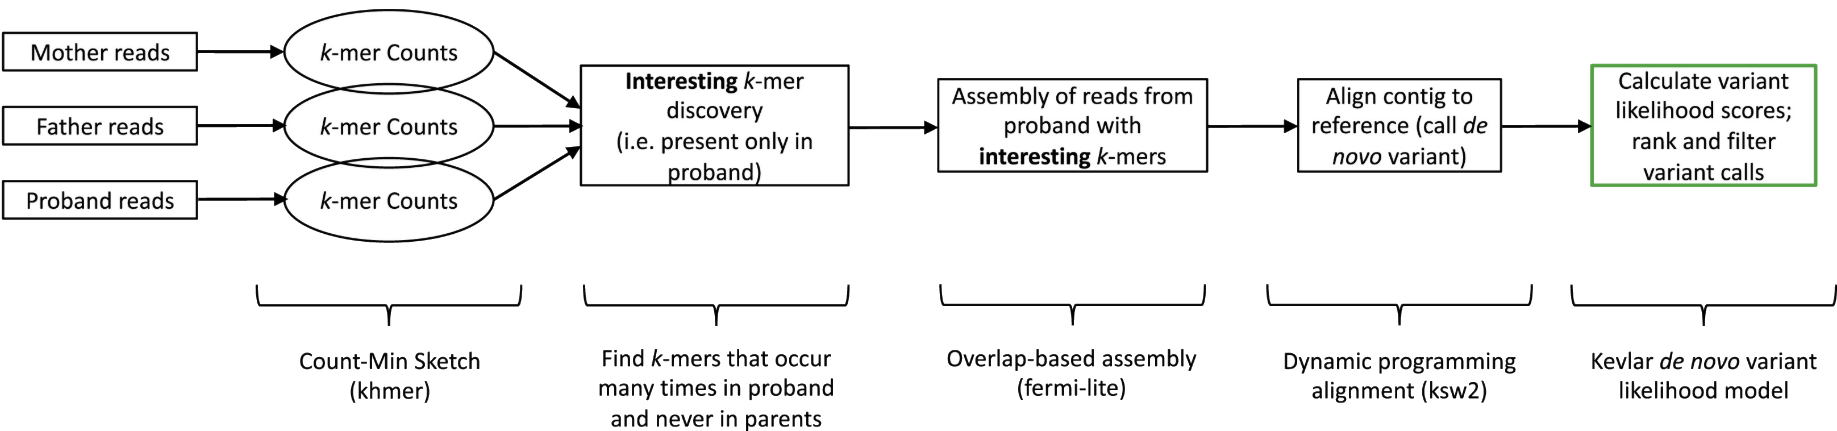
\includegraphics[scale=.27]{images/kevlar_pipeline.png}
  	\caption{Kevlar Pipeline}
  	\label{fig:kevlar_pipeline}
\end{figure}

\paragraph{Step 1} Prima di poter identificare nuovi \textit{k}-mer, è necessario contare la frequenza di ogni \textit{k}-mer all'interno di ogni genoma. Per fare ciò Kevlar memorizza un conteggio approssimativo dei \textit{k}-mer all'interno di Count-Min Sketch (vedi Sezione \ref{count-min}).  Viene quindi utilizzata per ogni campione una CM Sketch, la cui precisione dipende dalla dimensione e dal numero degli elementi distinti che vengono tracciati. In seguito, con l'utilizzo di una maschera di conteggio, se i \textit{k}-mer sono presenti nei genomi di riferimento e in un genoma di contaminanti (batteri, virus, ...) sono ignorati.

\paragraph{Step 2} Kevlar scansiona ogni read sequenziata dal probando e richiede le frequenze per campione di ciascun \textit{k}-mer alle Count-Min Sketch generate nella fase precedente. Se un \textit{k}-mer è presente con alta frequenza nel genoma figlio ed è assente dai genomi genitori è identificato come ``interessante". 

\paragraph{Step 3} Ogni read che contiene \textit{k}-mer interessanti viene filtrata prima di qualunque altra analisi. Questo filtraggio serve principalmente per due scopi: (1)dato il volume delle read che arriva a questo step, Kevlar è in grado di ricalcolare esattamente le frequenze di ogni \textit{k}-mer interessante nel probando e qualunque \textit{k}-mer il cui conteggio ``corretto'' non soddisfi più la frequenza di soglia viene scartato; (2) se, per qualunque ragione, dei \textit{k}-mer presenti nel genoma di riferimento e dei contaminanti non erano stati ignorati nel conteggio iniziale, questo filtraggio fornisce un'altra opportunità per scartarli. 

Dopo l'applicazione di questo filtraggio, qualunque read che non contiene \textit{k}-mer interessanti è scartata. Ci si aspetta ora che read interessanti condividano numerosi \textit{k}-mer interessanti: tramite questi è possibile raggruppare le read interessanti in insiemi disgiunti, ognuno rappresentante una mutazione. Per fare ciò viene definito un grafo di lettura $G$ nel seguente modo: ogni read contenente uno o più \textit{k}-mer interessanti è rappresentata da un nodo in $G$; una coppia di nodi è connessa da un arco se le rispettive read hanno uno o più \textit{k}-mer interessanti in comune. Grazie a questa formulazione, se due read condividono un \textit{k}-mer interessante, allora sono parte della stessa componente connessa di $G$. 

Per ogni componente connessa $p\in G$ viene assemblata la read corrispondente usando un algoritmo basato su overlap, implementato nella libreria Fermi-Lite e viene prodotto il cammino ottimale $C_p$ nel grafo (sottoforma di contig) adatto per effettuare chiamate delle varianti. Vengono successivamente selezionate delle sequenze obiettivo di riferimento per il contig $C_p$ denotate come $T_{C_p}$.

\paragraph{Step 4} Il contig $C_p$ viene allineato a ciascuna sequenza obiettivo $t \in T_{C_p}$ usando la libreria ksw2\footnote{\ ksw2 implementa la formulazione di Green di allineamento ed estensione globale della programmazione dinamica.}. 
Se sono presenti più sequenze obiettivo, viene mantenuto solo l'allineamento con il punteggio più alto. Quando un contig si allinea a più posizioni con lo stesso punteggio ottimale, tutti gli allineamenti ottimali vengono mantenuti per la chiamata della variante.
Prima di chiamare la variante, Kevlar allinea eventuali spazi vuoti all'estremità destra dell'allineamento per ridurre al minimo il numero di operazioni di allineamento. Successivamente, ispeziona il percorso di allineamento (rappresentato come una stringa \texttt{CIGAR}) di ciascun allineamento e verifica la corrispondenza con i pattern previsti. Allineamenti corrispondenti al pattern \verb|ˆ(\d+[DI])?\d+M(\d+[DI])?$| sono classificati come SNV e il blocco ``match" dell'allineamento viene scansionato per discrepanze tra il contig e l'obiettivo di riferimento. Qualsiasi discrepanza è segnalata come variante a singolo nucleotide. Gli allineamenti che corrispondono al pattern \verb|ˆ(\d+[DI])?\d+M\d+[ID]\d+M(\d+[DI])?$| sono invece classificati come indel. Oltre a segnalare il divario interno di questo allineamento come un indel, i blocchi ``match" fiancheggianti sono
scansionati anche per discrepanze tra il contig e il target da segnalare come putativi SNV. Qualsiasi allineamento che non corrisponde ai due pattern sopra descritti è designato come ``\texttt{no-call}'' ovvero non interpretabile, ed elencato nell'output con il contig corrispondente. 

\paragraph{Step 5} 

Per assegnare un punteggio e classificare le mutazioni \textit{de novo}, viene utilizzato un modello probabilistico che considera la frequenza dei \textit{k}-mer interessanti per calcolare la probabilità che siano \textit{de novo}, ereditati o semplicemente dei falsi positivi. Utilizzando queste probabilità, viene calcolato un punteggio per ogni mutazione \textit{de novo}, tramite dei rapporti di probabilità, e sulla base di questi ultimi viene calcolato tramite euristica un punteggio utile a classificare le mutazioni predette. Formalmente, l'euristica che sta alla base del calcolo del punteggio assegnato ad ogni variante è la seguente: \\
$$S_L = log \left(L\left(dn=1\right)\right) - max\left\lbrace log\left(L\left(ih=1\right)\right), log\left(L\left(fp=1\right)\right)\right\rbrace$$
\noindent
\\
dove $L\left(dn=1\right)$ è la probabilità che sia presente una nuova mutazione, $L\left(ih=1\right)$ è la probabilità che la mutazione sia ereditata e $L\left(fp=1\right)$ è la probabilità che una nuova mutazione possa essere un falso positivo.
%\textcolor{red}{io spiegherei un po' meglio qui, okay, assegna il punteggio e quindi? no con formule matematiche ma con le parole}

%e sono calcolate nel seguente modo:
%
%\begin{align*}
%L\left(ih=1\right) & = P\left( A_c,A_m, A_f \ | \ ih = 1 \right)\\
% & \approx \prod_{i=1}^n P\left( A_{c_i},A_{m_i}, A_{f_i} \ |\ ih = 1 \right)\\
% & = \prod_{i=1}^n \frac{P\left( ih = 1 \ | \ A_{c_i},A_{m_i}, A_{f_i} \right) P\left( A_{c_i},A_{m_i}, A_{f_i} \right)}{P\left( ih=1\right)}\\
%  & = \prod_{i=1}^n \frac{P\left( A_{c_i},A_{m_i}, A_{f_i} \right)}{P\left( ih=1\right)} \times P\left( ih = 1 \ | \ A_{c_i},A_{m_i}, A_{f_i} \right)
%\end{align*}
%
%\begin{align*}
%L\left(dn=1\right) & = P\left( A_c,A_m, A_f \ | \ dn = 1 \right)\\
% & = P\left( A_c,A_m, A_f \ | \ v_c = 0/1, v_m = 0/0, v_f = 0/0 \right)\\
% & = P\left( A_c \ | \ v_c = 0/1 \right) P\left( A_m \ | \ v_m = 0/0 \right) P\left( A_f \ | \ v_f = 0/0 \right)
%\end{align*}
%\begin{align*}
%L\left(fp=1\right) & = P\left( A_c,A_m, A_f \ | \ v_c = 0/0, v_m = 0/0, v_f = 0/0 \right)
%\end{align*}

\end{document}